\subsection*{Wi-Fi Physical Layer}
A constant change of the physical layer accompanies the further development of IEEE 802.11.
\textcite{sauter_wireless_2022} mentions that all new enhancements of the physical layer of IEEE 802.11 are backward
compatible with previous definitions of the standard.

According to the Author, IEEE 802.11 initially used DSSS and FHSS as modulation methods.
Since IEEE 802.11g the modulation method \ac{OFDM} can be used in the \SI{2.4}{\giga\hertz} frequency band.
The author explains \ac{OFDM} as follows. \ac{OFDM} divides the transmission channel into subcarriers with different
amplitudes, frequencies and phases.
Each subcarrier is orthogonal to another one, as they send the information ``Low``,
where only one other subcarrier is sending the information ``High``.


\subsubsection*{Symbol length}
The data is then sent as \ac{OFDM} symbols over the individual \ac{OFDM} subcarriers.
The distance between the ``Highs`` of the subcarriers is specified as subcarrier spacing and corresponds to the reciprocal
symbol length.
IEEE 802.11ax increased the \ac{OFDM} symbol length from \SI{3.2}{\micro\second} for IEEE 802.11n  to a maximum of \SI{12.8}{\micro\second} \cite{sauter_wireless_2022}.
This corresponds to a subcarrier spacing of \SI{312.5}{\kilo\hertz} and \SI{78.125}{\kilo\hertz} respectively \cite{sauter_wireless_2022}.

For the IEEE 802.11p and IEEE 802.11bd standards, a symbol length of \SI{6.4}{\micro\second} applies, corresponding to a subcarrier spacing of \SI{156.25}{\kilo\hertz} \cite{jacob_system-level_2020}.

The Fast Fourier Transform and Inverse Fast Fourier Transform are used to modulate and demodulate the transmitting bits.
With the reduction of subcarrier spacing, more subcarriers are created in the transmission channel,
so the Fast Fourier Transform size must be increased.

\textcite{kauffels_wireless_2002} adds, that \ac{OFDM} can be used in the \SI{5}{\giga\hertz} frequency band since IEEE 802.11a.
\subsubsection*{\acf{BW}}
The frequency bands were divided into channels in order to create several transmission channels.
This results in 13 channels in Europe in the frequency band of \SIrange{2.412}{2.482}{\giga\hertz} and 18 channels in the frequency band of \SIrange{5.180}{5.350}{\giga\hertz} and \SIrange{5.180}{5.350}{\giga\hertz}  \cite{sauter_wireless_2022}.
Transmission channels can be combined to enable higher data rates.
Every channel has a width called \ac{BW} and is specified in \si{\mega\hertz}.
The possible \ac{BW}s for the IEEE 802.11 standards are shown in \autoref{tab:BW}.
\begin{table}[!ht]
	\centering
	\begin{tabular}{>{\raggedright}p{2.2cm}p{2.50cm}p{2.55cm}p{2.50cm}}
		\toprule
		Standard & Channel \ac{BW}s\newline in \SI{2.4}{\giga\hertz}& Channel \ac{BW}s\newline in \SI{5}{\giga\hertz} &  Channel \ac{BW}s\newline in  \SI{5.9}{\giga\hertz}\\
		\midrule
		IEEE 802.11n \cite{sauter_wireless_2022}& \SI{20}{\mega\hertz},\SI{40}{\mega\hertz}  & \SI{20}{\mega\hertz},\SI{40}{\mega\hertz} & - \\
		\midrule
		IEEE 802.11ac \cite{noauthor_ieee_2021-1}& -  & \SI{20}{\mega\hertz},\SI{40}{\mega\hertz}, \SI{80}{\mega\hertz},\SI{160}{\mega\hertz} & - \\
		\midrule
		IEEE 802.11ax \cite{noauthor_ieee_2021}&\SI{20}{\mega\hertz},\SI{40}{\mega\hertz}  & \SI{20}{\mega\hertz},\SI{40}{\mega\hertz}, \SI{80}{\mega\hertz},\SI{160}{\mega\hertz} & - \\
		\midrule
		IEEE 802.11p \cite{jacob_system-level_2020}& - & - & \SI{10}{\mega\hertz} \\
		\midrule
		IEEE 802.11bd \cite{jacob_system-level_2020}& - & - & \SI{10}{\mega\hertz},\SI{20}{\mega\hertz} \\
		\bottomrule
	\end{tabular}
	\caption{Available \ac{BW}s for the IEEE 802.11 standards per frequency band.}
	\label{tab:BW}
\end{table}

IEEE 802.11ac and IEEE 802.11ax enable also the use of a discontinuous \ac{BW}, which combines two \SI{80}{\mega\hertz}
channel to a \SI{160}{\mega\hertz} \ac{BW} channel \cite{noauthor_ieee_2021}, \cite{noauthor_ieee_2021-1}.

While wider channels increase the theoretical data rate, \textcite{avallone_will_2021} mentions that narrower channels can
boost the signal's power spectral density and thus increase the transmission range.

\subsubsection*{\acf{MCS}}

In order to encode as many bits as possible on one \ac{OFDM} symbol, different \ac{MCS}s can be used.
The \ac{MCS}s for the IEEE 802.11 standards are based on \ac{PSK} or \ac{QAM}. \cite{kauffels_wireless_2002}.
The smallest \ac{MCS} is Binary - \ac{PSK} and encodes \SI{1}{\bit} per symbol.
IEEE 802.11ax has the most complex \ac{MCS} of \num{256} - \ac{QAM} IEEE 802.11ac to \num{1024} - \ac{QAM} and thus now encodes \SI{10}{\bit} per symbol \cite{afaqui_ieee_2017}.
In the \ac{V2X} range, so can \ac{MCS}s from binary-\ac{PSK} to \num{256}- \ac{QAM}.

An imaginary, theoretical transmission channel is usually specified as a square-wave signal in the frequency domain
with limits of both minimum and maximum amplitude and cut-off frequency. \textcite{kauffels_wireless_2002} defines
the roll-off factor as a cosine-shaped flattening of the square signal between 0 and 1.
In addition, the author points
out that \ac{QAM} can generate high roll-off factors so that signals interfere significantly more with adjacent channels.

In this regard, the author recommends setting the parameters in an \ac{OFDM} system so that first, the coding
rate and then the complexity of the \ac{MCS} is reduced in challenging transmission environments. The more bits a \ac{MCS} encodes
on a symbol, the more error-prone the correct decoding.

\subsubsection*{\acf{FEC}}

Nevertheless, bit errors can occur during transmission. In this regard, \cite{kauffels_wireless_2002}
mentions and explains \ac{FEC} as a technique to reduce bit errors during transmission. \ac{FEC} adds redundant bits
to the data. The receiver uses these redundant bits to check the integrity or correct errors of the received data.
The proportion of non-redundant transmission bits is defined in the \ac{CR}.

To achieve this, \ac{BCC} is used mandatory since the IEEE 802.11n standard \cite{afaqui_ieee_2017,syafei_performance_2009}
. \textcite{syafei_performance_2009} add that it is optionally possible to
use \ac{LDPC}.
The authors state that \ac{LDPC} can achieve a better channel capacity performance.
This impact is also confirmed by \textcite{afaqui_ieee_2017}, who point out that \ac{LDPC} also generates higher computational cost.

IEEE 802.11ax stations must support \ac{LDPC} when using the IEEE 802.11ax standard under
the following conditions \cite{afaqui_ieee_2017,noauthor_ieee_2021} :
\begin{itemize}
   \item The used bandwidth is greater than \SI{20}{\mega\hertz}
   \item The chosen \ac{MCS} is \num{1024}-\ac{QAM}
   \item More than four transmission channels are used for the transmission.
\end{itemize}
IEEE 802.11ax achieves \ac{CR} of \nicefrac{1}{2}, \nicefrac{2}{3}, \nicefrac{3}{4}, and \nicefrac{5}{6} \cite{noauthor_ieee_2021}.
Similarly, IEEE 802.11p uses the \ac{BCC} technique, which has been superseded by \ac{LDPC} in its successor
IEEE 802.11ax \cite{jacob_system-level_2020,krief_analysis_2020}.
\textcite{krief_analysis_2020} argue that this step was important, as \ac{LDPC} offers better error correction
possibilities for higher communication ranges greater than \SI{50}{\metre}.

Together with the \ac{MCS}, the \ac{FEC} \ac{CR} form a physical layer specification, which is named after the specific standard.
For IEEE 802.11ax, this results in the HE-MCS values in \autoref{tab:HEMCS}.

\begin{table}[!ht]
   \centering
   \begin{tabular}{>{\raggedright}p{2cm}p{3cm}p{2cm}}
      \toprule
      HE-MCS index & \acf{MCS} & \acf{CR} \\
      \midrule
      \num{0} & Binary \ac{PSK}& \nicefrac{1}{2}\\
      1 & Quadrature \ac{PSK}& \nicefrac{1}{2}\\
      2 & Quadrature \ac{PSK}& \nicefrac{3}{4}\\
      3 & \num{16}-\ac{QAM}& \nicefrac{1}{2}\\
      4 & \num{16}-\ac{QAM}& \nicefrac{3}{4}\\
      5 & \num{64}-\ac{QAM}& \nicefrac{2}{3}\\
      6 & \num{64}-\ac{QAM}& \nicefrac{3}{4}\\
      7 & \num{64}-\ac{QAM}& \nicefrac{5}{6}\\
      8 & \num{256}-\ac{QAM}& \nicefrac{3}{4}\\
      9 & \num{256}-\ac{QAM}& \nicefrac{5}{6}\\
      10 & \num{1024}-\ac{QAM}& \nicefrac{3}{4}\\
      11 & \num{1024}-\ac{QAM}& \nicefrac{5}{6}\\
      \bottomrule
   \end{tabular}
   \caption{\ac{MCS} and \ac{CR} for HE-\ac{MCS} values \cite{noauthor_ieee_2021}}
   \label{tab:HEMCS}
\end{table}

\begin{comment}
	{Wellenausbreitung, Überlagerungseffekte, Reflexsion, Reflexsion nicht bei Metall}

\end{comment}

\subsubsection*{\acf{GI}}
\textcite{pulimamidi_development_2007} explain the Guard Interval as a cyclic prefix of \ac{OFDM}symbols before
Inter Symbol Interference and through Inter Carrier Interference.
Inter Symbol Interference is caused by multipath delays, where the reflected delayed previous symbol can interfere
with the currently received symbol\cite{ravindranath_performance_2016}.
Similarly, Inter Carrier Interference is caused by time-varying channel resulting in a longer \ac{OFDM} symbol duration
\cite{van_duc_nguyen_intercarrier_2002}.


\textcite{pulimamidi_development_2007} explain how a guard interval can prevent these interferences.
Since the guard interval is to prevent possible interference on the following symbol, it must be at least long enough to catch all channel impulse responses with the resulting delay in the guard interval.
The guard interval is then removed again at the receiver.
This results in an attenuation of bandwidth which can be described
by the following formula:
\begin{equation}\label{eq:GI}
   \text{GI\_Bandwidth\_Attenuation} =
   \frac{
      \text{OFDM\_symbol\_duration} \times 100
   }{
      \text{OFDM\_symbol\_duration} + \text{GI}
   }
   \cdot
\end{equation}
Since IEEE 802.11n, a shortened \ac{GI} of \SI{400}{\nano\second} is usable, which increases the
maximum data rate from \SI{270}{\mega\bit\per\second} to \SI{300}{\mega\bit\per\second} compared to
the usual \ac{GI} of \SI{800}{\nano\second} \cite{sauter_wireless_2022}.
IEEE 802.11ax supports \ac{GI}s of \SI{800}{\nano\second}, \SI{1600}{\nano\second} and \SI{3200}{\nano\second} to
enable better protection against multipath effects in indoor and outdoor communications \cite{deng_ieee_2017}.

No condition for the use of the different \ac{GI} is mentioned in \cite{deng_ieee_2017}, \cite{rochim_performance_2020} , \cite{mozaffariahrar_survey_2022} or \cite{afaqui_ieee_2017}.
Moreover, the sources mentioned only specify a \ac{OFDM} symbol length of \SI{12.8}{\micro\second}.

Nevertheless, the standard IEEE 802.11ax \cite{noauthor_ieee_2021} specifies the following rules for using the different \ac{GI}s.
A \SI{1600}{\nano\second} \ac{GI} can only be used with a symbol length of \SI{6.4}{\micro\second}.
The same applies to a \ac{GI} of \SI{800}{\nano\second}, with the optional extension for use with a symbol length of \SI{3.2}{\micro\second}.
A \ac{GI} of \SI{3200}{\nano\second} can only be used for a symbol length of \SI{12.8}{\micro\second}.
\subsubsection*{\acf{DCM}}
To introduce additional robustness \ac{DCM} can be applied to the physical layer since
IEEE 802.11ax \cite{jacob_system-level_2020}, \cite{triwinarko_phy_2021}, \cite{noauthor_ieee_2021}.
\textcite{jacob_system-level_2020} describe \ac{DCM} as sending data twice over two coherent carriers.
At the receiver, the data copies are combined with the log-likelihood ratio.
Thus \ac{DCM} increases the probability of receiving the data.

\cite{noauthor_ieee_2021} provides a receiver minimum input sensitivity, which indicates until which RSS a packet is
received with a probability of \SI{90}{\percent}.
The receiver minimum input sensitivity for a \ac{BW} of
\SI{20}{\mega\hertz} is displayed in \autoref{fig:ReceiverSensitivityDCM}.
It demonstrates that when using \ac{DCM},
the receiver minimum input sensitivity can be lower than without using \ac{DCM}. The effect on the receiver minimum
input sensitivity increases as the HE-MCS value increases.
\begin{figure}%
	\centering
	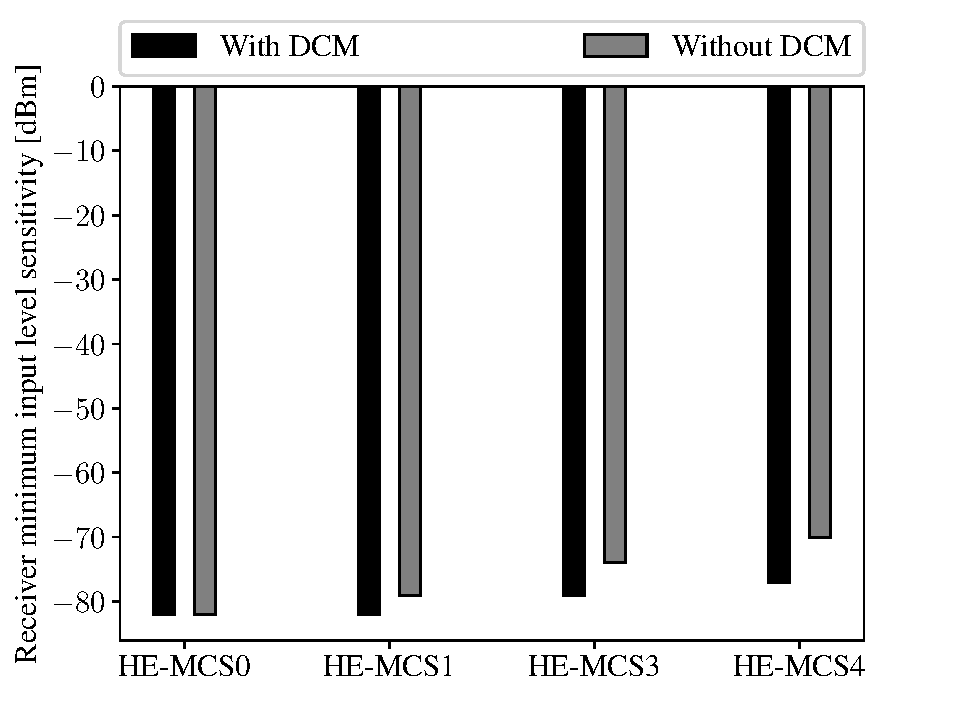
\includegraphics[width=0.95\textwidth]{figures/Receiver_minimum_DCM}
	\caption{Receiver minimum input level sensitivity for different HE-MCS values according to \cite{noauthor_ieee_2021}, where \ac{PER} is less than \SI{10}{\percent}}%
	\label{fig:ReceiverSensitivityDCM}%
\end{figure}

A similar development of the receiver minimum input sensitivity can also be observed for higher \ac{BW}, except
that the lowest value increases with \ac{BW}.

The higher probability of achieving data is achieved at the expense of the data rate.
The same amount of data now takes twice as long to transmit.

\cite{noauthor_ieee_2021} lists the theoretically possible data rates.
These reveal that the maximum achievable data rate with DCM is only half of the attainable data rate without DCM.

Support for \ac{DCM} is only optional in the IEEE 802.11ax standard and can only be used for HE-\ac{MCS}-\num{0},
HE-\ac{MCS}-\num{1}, HE-\ac{MCS}-\num{3} and HE-\ac{MCS}-\num{4} for \numrange{1}{2} spatial
transmission streams \cite{noauthor_ieee_2021}.

\textcite{jacob_system-level_2020} and \textcite{triwinarko_phy_2021} mention plans,
to allow using \ac{DCM} in the physical layer of IEEE 802.11bd.

\begin{comment}
	Allowed relative constellation error versus constellation size RMS error over subcarriers and Frequency
	
	Table 27-51—Receiver minimum input level sensitivity
	
	Table 27-52—Minimum required adjacent and nonadjacent channel rejection levels
	optional feature \cite{noauthor_ieee_2021}
	
	\ac{HE} SU \ac{PPDU} \ac{HE} \ac{ER} SU \ac{PPDU} not for GI 800 ns \cite{noauthor_ieee_2021}
\end{comment}

\subsubsection*{\acf{ER}}
Since IEEE 802.11ax, the \ac{ER} Mode exists, which defines the new \ac{HE} \ac{ER} SU \ac{PPDU} as physical lay\ac{ER} amendment
\cite{noauthor_ieee_2021,afaqui_ieee_2017} .
\textcite{deng_ieee_2017} explains that the \ac{HE} \ac{ER} SU \ac{PPDU} format is intended to extend the range of
a single station to access point transmission.
According to the authors, this is accomplished by the \ac{PPDU} containing a repetition of the HE-SIG-A field.

In addition, the authors explain that the preamble transmission power is boosted,
to guarantee reliable transmission for longer ranges.
The power-boost is limited to additional \SI{3}{\decibel}
in  \cite{noauthor_ieee_2021,jacob_system-level_2020}

The IEEE 802.11ax \cite{noauthor_ieee_2021} standard defines that the \ac{HE} \ac{ER} SU \ac{PPDU} format may only be used
when 20 Mhz transmissions with either 242-Resource Unit with HE-MCS-0 - HE-MCS-2 or 106-Resource Unit with HE-MCS-0 are used on a spatial stream.
In addition, one can use \ac{DCM}.
\textcite{sauter_wireless_2022} defines the Resource Unit as fragments of a wi-Fi channel. The number before the Resource Unit
indicates the number of subcarriers, which are part of the Resource Unit.

Optionally, the \ac{HE} \ac{ER} SU \ac{PPDU} may also be transmitted with a \ac{GI} of \SI{800}{\nano\second},
where an additional application of \ac{DCM} is forbidden.

\textcite{jacob_system-level_2020} and \textcite{triwinarko_phy_2021} add, that it is planned to use
the \ac{ER}  mode also in the IEEE 802.11bd standard.

\subsubsection*{\acf{MIMO}}
In order to further exploit the physical layer capabilities, the single transmitting and receiving antenna systems called Single-Input-Single-Output can be extended to \ac{MIMO} - systems.
\textcite{sauter_wireless_2022} describe the idea behind \ac{MIMO} as the usage of multiple transmit antennas and multiple receiving antennas. Spatial multiplexing is used so that the transmitted signals
from each antenna are reflected differently on objects and can thus be received from different directions at the receiver antennas.

The authors explain that since IEEE 802.11n, it is possible to use up to \num{4} MIMO streams.
This number was increased again to up to \num{8} MIMO streams in IEEE 802.11ax \cite{noauthor_ieee_2021}.
Since data can be sent simultaneously via each MIMO stream,
the theoretical data rate can thus increase proportionally depending on the usable streams.
The mechanism is called \ac{SU}-\ac{MIMO} \cite{noauthor_ieee_2021}.

\textcite{sauter_wireless_2022} mentions, that since IEEE 802.11ac it is possible to use Downlink \ac{MU}-\ac{MIMO},
which allows an \ac{AP} to transmit data to multiple \ac{STA} via different available \ac{MIMO} stream simultaneously.
According to the authors, \ac{MU}-\ac{MIMO} can increase the network throughput.
IEEE 802.11ax introduced \ac{MU}-\ac{MIMO} in the Uplink direction \cite{noauthor_ieee_2021}, where multiple \ac{STA} can transmit data simultaneously to the \ac{AP} via different available \ac{MIMO} streams.
MU-\ac{MIMO} DCM can also be applied in IEEE 802.11ax \cite{noauthor_ieee_2021}.

Another \ac{MIMO} technique is \ac{OFDMA}, which can be utilized since IEEE 802.11ax \cite{noauthor_ieee_2021, avallone_will_2021, omar_survey_2016}.
\textcite{avallone_will_2021} explains, \ac{OFDMA} enables an \ac{AP} to transmit data to multiple \ac{STA} simultaneously by dividing the available bandwidth into \ac{RU} and assigning each \ac{RU} to a \ac{STA}.
The authors add, that \ac{OFDMA} can be used in both the uplink and downlink direction.
The \ac{AP} can choose the best suited \ac{RU} for each \ac{STA} and thus increase the Signal-to-Interference-plus-Noise Ratio \cite{khorov_tutorial_2019}
\textcite{behara_performance_2022} adds, that \ac{OFDMA} is designed to improve the per-user throughput in high-density networks, e.q.
stadiums, airports or public transportation systems.

\subsubsection*{\acf{STBC}}
\textcite{abbas_efficient_2016} further explains that \ac{MIMO} spatial streams can be utilized to enhance the
quality of the received signal.
The Technology is called \ac{STBC}.
\textcite{santumon_space-time_2012} explains as follows.
\ac{STBC} is a technique used in Wi-Fi networks to improve the reliability and robustness of wireless communications.
\ac{STBC} encodes multiple redundant copies of data at the transmit side, which are transmitted in different spatial streams to
reduce fading and interference effects.
At the receiver side, these multiple copies are combined using a maximum likelihood detector
to retain a high-quality signal and decrease the \ac{PER}.


Here, \textcite{stamoulis_impact_2003} has investigated the potential effect of \ac{STBC} on Wi-Fi.
Their simulations showed that\ac{STBC} increase the range and robustness for IEEE 802.11a.
In addition, the authors concluded that \ac{STBC} increases the \ac{SNR} in nearly all cases at the same throughput or
even allows higher \ac{MCS} values to be used,
thus allowing a higher throughput at the same \ac{SNR}.
This results in \ac{STBC} improving the reliability and robustness of wireless communications.

\textcite{ghosh_error_2014} analyzed the error rate performance for an increased number of used antennae and found
that a lower bit error rate can be achieved
when increasing the number of transmit antennas with \ac{STBC}.

\textcite{gast_80211n_nodate} and \textcite{sauter_wireless_2022} mention, that \ac{STBC} can extend the signal range
due to the increased robustness.


IEEE 802.11ax stations can optionally use \ac{STBC} the following conditions \cite{noauthor_ieee_2021}:
\begin{itemize}
	\item DCM is not applied
	\item The number of spatial streams is \num{2}
	\item The \ac{GI} is not \SI{0.8}{\nano\second} and the symbol length is not \SI{12.8}{\micro\second}
\end{itemize}

\cite{gast_80211n_nodate} states that \ac{STBC} is only supported in one-fifth of the Wi-Fi-certified devices.



\begin{comment}
In addition to the physical layer parameters already discussed, other technologies can be applied. IEEE 802.11ax
Beamforming
OFDMA
Group addressed frames
HE Capabilities nur so gut, wie das schlechteste Glied
\end{comment}
